\chapter{波、量子化されたモード、生成演算子}

\section{波、場、複素指数関数}

量子場の理論は素粒子物理学の基本的な道具である。量子場について初歩的な説明を与える前にさえ、波と粒子を結びつける数学的事実をまとめておくと有用である。波はすでに一つの場の配位である。場は空間の点ごとに変化し、波とはそれらの値が振動し伝播する配位である。量子力学は、そのような波と粒子の間の結びつきを与える。

ここでは量子力学と特殊相対性理論を前提知識とする。当面の目的は、素粒子物理学に必要な事柄を復習することであり、どちらの科目の講義を置き換えることではない。

指数関数は比例的な増加によって特徴づけられる。もし
\begin{equation}
f(x)=e^{\alpha x},
\end{equation}
ならば
\begin{equation}
\frac{df}{dx}=\alpha f.
\end{equation}
である。小さな区間では、増加はすでに存在する量に比例する。ペトリ皿の中で増殖する個体群はよく知られた描像を与える。存在する生物が多いほど、繁殖に利用できる生物が多くなり、増加率は個体群そのものに比例する。\(e^{\alpha x}\) に全体の定数を掛けても、この定義的な性質は変わらない。

サインとコサインは、増加する代わりに振動する。それらは1周期の4分の1だけずれた同じ曲線であり、微分はそれらを互いに移り合わせる。
\begin{align}
\frac{d}{dx}\sin(kx)&=k\cos(kx),\\
\frac{d}{dx}\cos(kx)&=-k\sin(kx).
\end{align}
どちらの関数も単独では指数関数ではない。その導関数が他方の関数に比例するからである。複素数の組み合わせは指数関数の性質をもつ。\(i^2=-1\) として、
\begin{align}
\frac{d}{dx}\bigl(\cos(kx)+i\sin(kx)\bigr)
&=-k\sin(kx)+ik\cos(kx)\\
&=ik\bigl(\cos(kx)+i\sin(kx)\bigr).
\end{align}
したがって
\begin{equation}
e^{ikx}=\cos(kx)+i\sin(kx).
\end{equation}
である。この恒等式が繰り返し現れるのは、サインとコサインが波のような振動を記述するからである。\(x\) が空間座標であるとき、この関数は空間を通して振動する。引数が時間であるとき、それは時間の中で振動する。

\section{振動数、波長、光子の運動量}

通常の振動数 \(f\) は、毎秒の完全な周期の数である。一周期とは一回の完全な振動を意味する。角振動数は同じ運動をラジアン毎秒で測ったものである：
\begin{equation}
\omega=2\pi f.
\end{equation}
この二つの表記は同じ振動数を表している。計算から不要な \(2\pi\) の因子を排除するために両者を使い分けるが、その因子が完全に消えるわけではない。

波長 \(\lambda\) は、空間における一つの完全な周期が占める距離である。波が速さ \(v\) で伝播するなら、一周期あたりの距離に毎秒の周期数を掛けたものが伝播速度となる：
\begin{equation}
\lambda f=v.
\end{equation}
真空中の光では \(v=c\) であるから、
\begin{equation}
\lambda f=c.
\end{equation}
となる。音波では右辺は音速であり、水面波では対応する水面波の速度である。したがって \(c\) が現れることは光についての主張であり、すべての波に共通の定義ではない。

量子力学はプランク定数を2つの記法で導入する。
\begin{equation}
\hbar=\frac{h}{2\pi}.
\end{equation}
\(h\) から \(\hbar\) への変更は、\(2\pi\) の因子をある方程式から別の方程式へ移すだけである。

次元をもつ定数の数値は、それを表すのに用いる単位に依存する。メートル、秒、キログラムは人間の尺度に基づく約束であり、日常的な長さと時間に便利である。腕の長さに匹敵する伝統的な単位は布や縄に有用であった。メートルに至る正確な歴史的経路が何であれ、この特定の人間の尺度を選ぶ基本原理は存在しない。SI単位では、
\begin{equation}
\begin{aligned}
h &\simeq 6.6\times10^{-34}\ \mathrm{J\,s},
&\hbar &\simeq 1.1\times10^{-34}\ \mathrm{J\,s},\\
c &\simeq 3\times10^8\ \mathrm{m\,s^{-1}}.
\end{aligned}
\end{equation}
である。これらの数値の要点は、従来の単位におけるその尺度にある。プランク定数は極めて小さく、光速は極めて大きい。

あるモードの一つの量子はエネルギー
\begin{equation}
E_{\text{one quantum}}=\hbar\omega=hf.
\end{equation}
をもつ。これは一つの光子のエネルギーであり、任意の古典電磁波の全エネルギーではない。可視光の振動数はおよそ \(10^{15}\) サイクル毎秒であるから、典型的な光学光子のエネルギーはおよそ
\begin{equation}
E_\gamma\sim 10^{-19}\ \mathrm{J}.
\end{equation}
となる。これほど速い光学的振動であっても、\(h\) が非常に小さいため、量子一つあたりのエネルギーはごく小さい。したがって巨視的な量の光学エネルギーには膨大な数の光子が含まれる。

エネルギーと運動量はどちらも保存されるため、特別な注意に値する。それらは有用な簿記の量である。過程に入る全エネルギーと運動量は、それから出る全エネルギーと運動量によって釣り合わなければならない。運動量はベクトルであり、運動の方向を指す。光よりはるかに遅く運動する粒子では、
\begin{equation}
\vec p=m\vec v.
\end{equation}

次に、多くの方向へ分散するのではなく、一つの方向に沿ってコリメートされた電磁放射を考えよう。その運動量はビームに沿って向いている。非相対論的な式を光子に適用することはできない。\(m\) は静止質量を意味するが、光子の静止質量はゼロだからである。それでもなお、有用な次元の記憶法がある。もし誰かが\emph{不適切にも}光子に、あたかも質量であるかのように量 \(E/c^2\) を割り当て、次に \(v=c\) を代入すると、
\begin{equation}
mv\longrightarrow \frac{E}{c^2}c=\frac{E}{c}.
\end{equation}
が得られる。この操作はたまたま正しい答えを与え、単位も正しくするが、光子が静止質量 \(E/c^2\) をもつという正当な論証ではない。コリメートされた放射についての実際の相対論的記述は
\begin{equation}
|\vec p|=\frac{E}{c}.
\end{equation}
である。この式は大きさを与える。向きは放射が進む向きである。

一つの光子について、
\begin{align}
|\vec p_\gamma|
&=\frac{E_\gamma}{c}
=\frac{hf}{c}.
\end{align}
光について、
\begin{equation}
\lambda f=c,
\qquad
\frac{f}{c}=\frac{1}{\lambda},
\end{equation}
したがって
\begin{equation}
|\vec p_\gamma|=\frac{hf}{c}=\frac{h}{\lambda}.
\end{equation}

\begin{figure}[t]
\centering
\includegraphics[width=0.56\textwidth]{lecture_02_figure_02.png}
\caption{光について、\(\lambda f=c\) および \(f/c=1/\lambda\) であり、これらは \(|\vec p_\gamma|=h/\lambda\) を得るために用いられる関係である。}
\lectureframe{00:21:39}
\end{figure}

波長が短いほど、光子の運動量は大きい。これは素粒子物理学にとって最も重要な量子的事実の一つである。小さな対象を調べるには短波長のプローブが必要であり、その短波長の代償は大きな運動量である。

\begin{classroomqa}
\lecturetimestamp{00:22:23}
\audiencequestion{\(E=\hbar\omega\) は基本的なのか、それともより深い原理から導かれるのか。}
\lecturerresponse{それは調和振動子の量子力学から従う。その結果はここでは証明を繰り返さずに用いる。以下で展開する振動子の言葉が、それにとってより深い枠組みを与える。}
\end{classroomqa}


\section{波の振幅と光子数}

\begin{classroomqa}
\lecturetimestamp{00:23:10}
\audiencequestion{光子の言葉で、波の振幅は何を意味するのか。}
\lecturerresponse{同じ波長と振動数をもつが振幅が異なる二つの波、たとえば \(\sin(kx)\) と \(A\sin(kx)\) を比較しよう。古典的には、固定された領域内のエネルギーは振幅の二乗に比例する。量子力学的には、\(n\) 個の光子を含むモードはエネルギー \(n\hbar\omega\) をもつ。したがって、振動数、領域、規格化を固定すると、振幅は桁の程度で \(\sqrt n\) のように増大する。}
\end{classroomqa}

この二つの波は振動のパターンが同一である。一方が他方より単に強いだけである。\footnote{この模式図は 00 における波の比較に対応する。23：47--00：24：28。}

\begin{figure}[t]
\centering
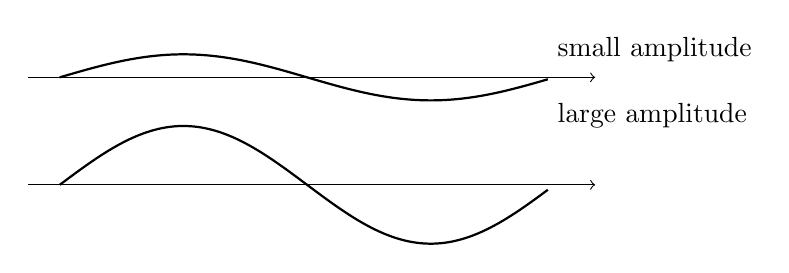
\begin{tikzpicture}[x=1cm,y=0.65cm]
\draw[->] (-0.4,0) -- (6.8,0);
\draw[->] (-0.4,-2.1) -- (6.8,-2.1);
\draw[thick] plot[domain=0:6.2,samples=120] (\x,{0.45*sin(\x r)});
\draw[thick] plot[domain=0:6.2,samples=120] (\x,{-2.1+1.15*sin(\x r)});
\draw (6.2,0.55) node[right]{small amplitude};
\draw (6.2,-0.75) node[right]{large amplitude};
\end{tikzpicture}
\caption{波長と振動数が等しいが振幅が異なる波。}
\end{figure}

固定された量の波について、
\begin{equation}
E_{\text{wave}}\propto A^2.
\end{equation}
電磁波については、これは場のエネルギーが場の強さの二乗に比例するというよく知られた記述である。同じモードが \(n\) 個の光子を含むならば、
\begin{equation}
E_{\text{wave}}=n\hbar\omega.
\end{equation}
したがって、モード、振動数、規格化、領域を固定すると、
\begin{equation}
A^2\propto n\hbar\omega,
\qquad
A\propto\sqrt n\quad\text{at fixed }\omega.
\end{equation}
厳密な規格化を主張しているのではない。含まれる波の量が重要である。それ以外は一様な波の長さを二倍にすると、局所的な振幅を変えずに全エネルギーが変わる。したがって、この比例関係は、一つの波長のような固定された領域について理解すればよい。

さらに、量子に固有の限定がある。振幅と位相の両方に厳密な古典値を割り当てることはできない。したがって、``一つの光子の振幅は何か'' という問いは、完全に鋭い古典場を求めるものであるならば曖昧である。それでも \(n=1\) と置くと、妥当な桁の尺度が得られる。

\begin{classroomqa}
\lecturetimestamp{00:28:25}
\audiencequestion{電磁波の図における縦方向の変位は、光子の空間内の位置を表すのか。}
\lecturerresponse{いいえ。伝播軸は空間的であるが、縦座標は電場または磁場の値を表す。運動量は伝播軸に沿って向いており、描かれた場の振幅に沿ってではない。}
\end{classroomqa}

波は任意の空間方向に伝播しうるが、よく知られた正弦波の図はその水平軸だけを空間座標として用いる。もう一方の描かれた方向は場の強さを記録する。

\begin{classroomqa}
\lecturetimestamp{00:29:37}
\audiencequestion{述べられた光子数は、波の一つの波長または周期の中で数えられているのか。}
\lecturerresponse{一つの波長のような固定された領域を選べばよい。これが、この関係が比例にすぎない理由である。全エネルギーと光子数は、波のどれだけが含まれるかにも依存する。同じ振幅で二つ、三つ、または四つの波長は、一つの波長よりもそれに応じて多くのエネルギーを含む。}
\end{classroomqa}

\begin{classroomqa}
\lecturetimestamp{00:30:17}
\audiencequestion{単一光子の振幅は無意味なのか。}
\lecturerresponse{それは\(n=1\)と置くことで得られる桁程度の記述としてのみ意味を持つ。電磁モードでは、電場と磁場の情報が共役な位置と運動量の情報に類似した役割を果たすため、量子不確定性が古典的振幅をどれほど鋭く割り当てられるかを制限する。桁程度の関係は依然として有用である。}
\end{classroomqa}

これらの問いはすでに量子場の理論へと導く。そこでは場の変数と粒子数の関係を精密に述べることができる。今のところは比例関係で十分である。

\section{一般的な量子関係と遅い物質波}

光子に対して導入された公式のうち、はるかに一般的に適用できるものもあれば、そうでないものもある。電子に移る前にそれらを整理しておく価値がある。

\begin{figure}[t]
\centering
\includegraphics[width=0.82\textwidth]{lecture_02_figure_03.png}
\caption{波の定義と、光子および非相対論的運動量の関係を、それぞれの適用範囲によって比較したもの。}
\lectureframe{00:31:52}
\end{figure}

\(f\)、\(\omega=2\pi f\)、\(\lambda\)の定義は一般的に適用できる。量子関係
\begin{equation}
E=\hbar\omega=hf
\end{equation}
もまた、本稿の議論において一般的である。対照的に、\(c\)を含む公式、たとえば\(\lambda f=c\)や\(|\vec p|=E/c\)は、光速で進む波に適用される。公式\(\vec p=m\vec v\)は、光よりもはるかに遅く進む粒子に適用される。これらの限界の間にある相対論的な運動には、まだ必要とされない補間が必要である。

運動量--波長関係は光子の例を経ても生き残る：
\begin{equation}
p=\frac{h}{\lambda}.
\end{equation}
ここで\(p\)は、\(\lambda\)を正の波長ととったときの大きさを表す。方向は別に与えることができる。

\begin{figure}[t]
\centering
\includegraphics[width=0.74\textwidth]{lecture_02_figure_04.png}
\caption{光子の運動量\(|\vec p_\gamma|=hf/c=h/\lambda\)、そして一般的なド・ブロイ関係へと導く。}
\lectureframe{00:33:32}
\end{figure}

電子、原子核、さらにはボウリングの球でさえも波と関連付けることができる。電子の干渉はその事実の一つの現れである。電子波を\(\psi\)と書く。ゆっくり動く電子に対して\(\lambda f=c\)に代わるものは何か。欠けている要素は、エネルギーと運動量の間の非相対論的関係である。

運動エネルギーと運動量から始める：
\begin{align}
E&=\frac12 mv^2,\\
p&=mv,
\qquad
v=\frac{p}{m}.
\end{align}
最後の関係を最初の式に代入すると
\begin{align}
E
&=\frac12m\left(\frac{p}{m}\right)^2\\
&=\frac{p^2}{2m}.
\end{align}
質量は\(\frac12 mv^2\)では分子にあり、\(p^2/(2m)\)では分母にある。この配置は混同しやすく、再導出するのに有用である。

次に一般的な量子関係
\begin{equation}
E=hf,
\qquad
p=\frac{h}{\lambda}.
\end{equation}
を用いる。単一の遅い粒子に対して、
\begin{align}
hf
&=\frac{p^2}{2m}\\
&=\frac{1}{2m}\left(\frac{h}{\lambda}\right)^2\\
&=\frac{h^2}{2m\lambda^2}.
\end{align}
\(h\)で割ると
\begin{equation}
f=\frac{h}{2m\lambda^2}.
\end{equation}

\begin{figure}[t]
\centering
\includegraphics[width=0.64\textwidth]{lecture_02_figure_05.png}
\caption{遅い粒子に対して、\(E=p^2/(2m)\)と\(p=h/\lambda\)から\(f=h/(2m\lambda^2)\)が得られる。}
\lectureframe{00:37:47}
\end{figure}

光に対しては、
\begin{equation}
f\propto\frac{1}{\lambda},
\end{equation}
一方、遅い物質に対しては、
\begin{equation}
f\propto\frac{1}{\lambda^2}.
\end{equation}
第二の関係を単独で暗記する必要はない。それは常に\(E=p^2/(2m)\)、\(E=hf\)、\(p=h/\lambda\)から再構成できる。原子中をゆっくり動く電子に対して、それは対応するSchr\"odinger波の振動数を与える。

\begin{classroomqa}
\lecturetimestamp{00:38:35}
\audiencequestion{非相対論的な振動数--波長関係は電子以外の粒子にも適用されるか。}
\lecturerresponse{はい。それは光よりもはるかに遅く動く任意の粒子に適用される。遅い極限と光的極限の間の相対論的補間は別の主題である。}
\end{classroomqa}

\begin{classroomqa}
\lecturetimestamp{00:38:55}
\audiencequestion{ニュートリノにはどの関係が適用されるか。}
\lecturerresponse{ニュートリノの速さによる。自然界で出会うほとんどのニュートリノは光速に非常に近く動くので、光的関係が良い近似となる。光よりもはるかに遅く動くニュートリノは、代わりに非相対論的関係に従うであろう。}
\end{classroomqa}

\editorialnote{ニュートリノの質問の直後に行われた短い聴衆とのやり取りは振幅、量子、および異なる電子波長に関するものであるが、その文言は損傷がひどく安全に復元できない。復元可能な応答は、振幅と異なる波長の量子の間の一般的な関係を先延ばしにしている。}

\begin{classroomqa}
\lecturetimestamp{00:39:56}
\audiencequestion{\(20\,\mathrm{keV}\)加速器からの電子は遅いのか相対論的なのか。}
\lecturerresponse{それは遅いものとして扱われる。\(c=1\)とする単位系では、質量、エネルギー、運動量を同じ単位で表すことができる。電子の静止エネルギー尺度はおよそ\(0.5\,\mathrm{MeV}\)である一方、\(20\,\mathrm{keV}\)ははるかに小さい。同等に、非相対論的運動量の基準は\(p\ll mc\)である。}
\end{classroomqa}

この例におけるエネルギー比較は
\begin{equation}
K=20\,\mathrm{keV}\ll m_ec^2\simeq0.5\,\mathrm{MeV}.
\end{equation}
\editorialnote{出典箇所 00:39:56--00:41:40 は \(20\,\mathrm{keV}\) を加速器のエネルギーとして導入し、その後、相対論的判定基準を運動量と静止質量の比較として表現している。運動エネルギーと運動量の判定基準を別々に書くことで、引用されたエネルギーを運動量と同一視することを避けつつ、述べられている非相対論的結論を保つことができる。}

\section{位相速度、群速度、分散}

\begin{classroomqa}
\lecturetimestamp{00:41:46}
\audiencequestion{振動数に波長を掛けると電子波の速度が得られるか。}
\lecturerresponse{それは位相速度を与えるのであって、電子に割り当てられる速度ではない。局在した波束は、その内部の山と谷の運動を記述する位相速度と、包絡線の運動を記述する群速度の両方をもつ。群速度が粒子の運動と同一視される。}
\end{classroomqa}

波束は局所的には正弦または余弦のように見えるが、包絡線によって閉じ込められている。それが動くとき、包絡線とその内部の山は同じ速さで動く必要はない。\footnote{この模式図は 00:42:34--00:44:11 における波束の議論に従っている。}

\begin{figure}[t]
\centering
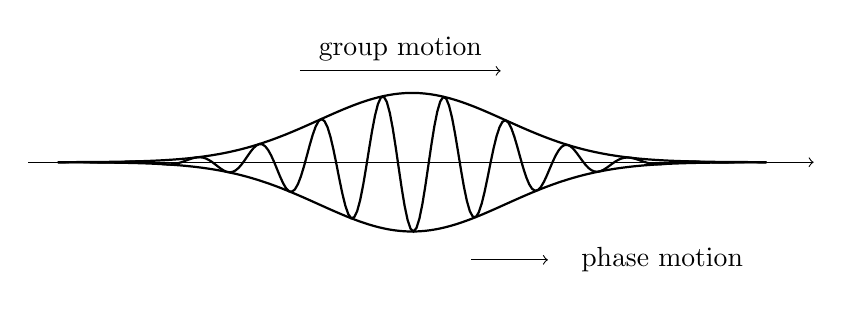
\begin{tikzpicture}[x=0.75cm,y=0.8cm]
\draw[->] (-0.5,0) -- (12.8,0);
\draw[thick] plot[domain=0:12,samples=140] (\x,{1.10*exp(-0.20*(\x-6)^2)});
\draw[thick] plot[domain=0:12,samples=140] (\x,{-1.10*exp(-0.20*(\x-6)^2)});
\draw[thick] plot[domain=0:12,samples=240] (\x,{1.10*exp(-0.20*(\x-6)^2)*sin(6*\x r)});
\draw[->] (4.1,1.45) -- (7.5,1.45);
\draw (5.8,1.8) node{group motion};
\draw[->] (7.0,-1.55) -- (8.3,-1.55);
\draw (8.7,-1.55) node[right]{phase motion};
\end{tikzpicture}
\caption{包絡線と内部の位相が一般に異なる速度で動く局在した波束。}
\end{figure}

位相速度は、単色成分の山、谷、その他の固定された位相の速度である。非相対論的分散関係では、
\begin{equation}
v_\phi=f\lambda=\frac{h}{2m\lambda}.
\end{equation}
これは波長に依存する。したがって異なる波長成分は異なる位相速度をもち、そのため山は波束の中を移動でき、波束は分散しうる。群速度は波束全体の速度であり、粒子と同一視されるのはこちらである。

単純な特別の場合がある。すべての波長成分が同じ速度で動くならば、位相速度と群速度は一致する。真空中の光はこの性質をもつ。すなわちすべての波長が \(c\) で伝播する。低速粒子の関係はそうではない。その \(f\lambda\) は \(\lambda\) とともに変化する。

方程式
\begin{equation}
f=\frac{h}{2m\lambda^2}
\end{equation}
は、少し姿を変えた自由 Schr\"odinger 方程式である。振動数は平面波の時間依存性を指定し、波長はその空間依存性を指定し、Schr\"odinger 方程式が両者を関係づける。逆に、確定した振動数と確定した波長をもつ波を自由 Schr\"odinger 方程式に代入すると、この分散関係が再現される。

\begin{classroomqa}
\lecturetimestamp{00:47:02}
\audiencequestion{位相速度は光速を超えうるか。}
\lecturerresponse{超えうる。位相速度は情報を運ばない。情報と局在した波束は群速度で伝播するので、超光速の位相速度があっても超光速の信号伝達は許されない。}
\end{classroomqa}

\section{有限空間と離散運動量}

最終的な関心は無限空間における波にあるが、有限系の方が安全な出発点である。無限はコンピュータが直接保存したり操作したりできるものではない。まず有限系について方程式を定式化し、その後ではじめてその大きさがいくらでも大きくなる極限をとる。この習慣は量子力学、量子場の理論、素粒子物理学を通じて有用である。

空間一次元から始めても、本質的なものは何も失われない。波はバイオリン弦の上に、揺さぶられているロープの上に、あるいは抽象的な一次元世界に存在してもよい。最も明らかな有限系は、反射端をもつ長さ\(L\)の線分である。波は端まで進み、反射し、そして戻ってくる。これは完全に正当な反射境界条件であるが、一つの不便さがある。すなわち、波の系の内部で運動量が保存されないのである。右向きに進む波は右向きの運動量を運ぶ。反射後には、それは左向きの運動量を運ぶ。境界が力積を与え、その差を吸収したのである。

反射端における運動量の反転は模式的に表せる。\footnote{この模式図は 00:49:24--00:51:08 における反射境界の議論に従っている。}

\begin{figure}[t]
\centering
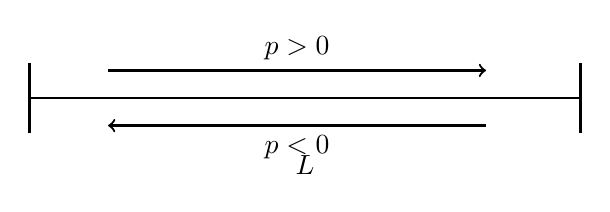
\begin{tikzpicture}[x=1cm,y=1cm]
\draw[thick] (0,0) -- (7,0);
\draw[very thick] (0,-0.45) -- (0,0.45);
\draw[very thick] (7,-0.45) -- (7,0.45);
\draw[->,thick] (1.0,0.35) -- (5.8,0.35) node[midway,above]{\(p>0\)};
\draw[->,thick] (5.8,-0.35) -- (1.0,-0.35) node[midway,below]{\(p<0\)};
\draw (3.5,-0.85) node{\(L\)};
\end{tikzpicture}
\caption{有限線分の端における反射は進行波の運動量を反転させる。}
\end{figure}

運動量を保ちながら系を有限にする別の方法がある。線分の両端点を同一視するのである。結果を円として描くことは可能だが、2次元に埋め込まれた文字通りの円は必要ない。数学的な言明は単に、座標が周期的であるということである。すなわち全距離 \(L\) だけ進んだ後、同じ点に戻る。

\begin{figure}[t]
\centering
\includegraphics[width=0.72\textwidth]{lecture_02_figure_06.png}
\caption{周期的同一視を導入するために用いられる、全長\(L\)の一次元経路。}
\lectureframe{00:51:21}
\end{figure}

端点の同一視は、次の模式図で明示される。\footnote{この模式図は00における周期的同一視の議論に従っている：51：09--00：52：37。}

\begin{figure}[t]
\centering
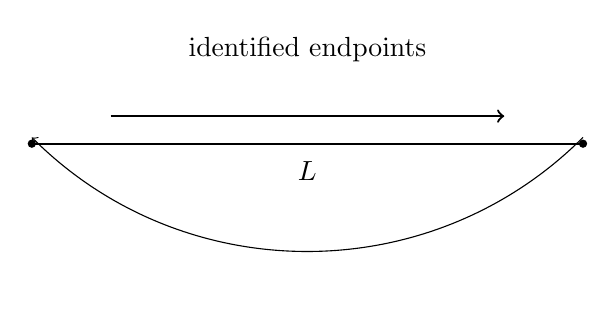
\begin{tikzpicture}[x=1cm,y=1cm]
\draw[thick] (0,0) -- (7,0);
\fill (0,0) circle (1.5pt);
\fill (7,0) circle (1.5pt);
\draw[->,thick] (1.0,0.35) -- (6.0,0.35);
\draw (3.5,-0.35) node{\(L\)};
\draw[->,bend left=45] (7,0.08) to (0,0.08);
\draw (3.5,1.2) node{identified endpoints};
\end{tikzpicture}
\caption{長さ\(L\)の経路の端点を同一視して得られる周期的な一次元空間。}
\end{figure}

右へ進む波は、やがて図示された端点に達すると始点に現れ、そのまま右へ進み続ける。左へ進む波も同様に左へ進み続ける。波が反射する特別な端点は存在しないため、運動量は反転しない。周期的空間は体積を有限にし、運動量を保存するが、重要な帰結を伴う。すなわち、許される運動量が離散的になるのである。

全長の中に整数個の波長が収まらなければならない。非定数モードに対して、
\begin{equation}
\lambda_{|N|}=\frac{L}{|N|},
\qquad |N|=1,2,3,\ldots .
\end{equation}
したがって波長の大きさは\(L\)、\(L/2\)、\(L/3\)などでありうる。\(L/\sqrt{2}\)のような選択は収まらない。一周した後、波は誤った位相で戻ることになり、始点での値と一致しなくなるからである。

\(p=h/\lambda\)を用いると、\(|N|\)番目の非定数モードの運動量の大きさは
\begin{equation}
|p_N|=\frac{|N|h}{L}.
\end{equation}
両方向と定数モードを曖昧さなく含めるには、モードのラベルを符号付きにするのが便利である：
\begin{equation}
p_N=\frac{Nh}{L},
\qquad N=0,\pm1,\pm2,\ldots .
\end{equation}
正と負の\(N\)は反対の伝播方向を表す。\(N=0\)モードは定数であり、運動量はゼロである。\(h/\lambda\)に代入すべき有限の波長は存在しない。したがって、基本的な運動量の間隔は\(h/L\)である。

巨視的な\(L\)に対しては、\(h\)も\(1/L\)もこの間隔を極めて小さくするため、許される値は非常に密な集合をなし、ほとんど連続に見える。それでも、円形の針金に拘束されたビーズはまさにこの離散的なスペクトルをもつ。

\begin{classroomqa}
\lecturetimestamp{00:58:27}
\audiencequestion{量子化される量は波の全運動量なのか、それとも一周期に対応する運動量なのか。}
\lecturerresponse{この記述は各量子の運動量に当てはまる。各量子は許された離散的な運動量のいずれかをもつ。したがって、任意の量子の集まりの全運動量もまた、基本単位\(h/L\)の整数倍である。}
\end{classroomqa}

\begin{classroomqa}
\lecturetimestamp{00:59:22}
\audiencequestion{なぜ波は一周した後で同じ値に戻らなければならないのか。}
\lecturerresponse{同一視された端点は同じ物理的点であるため、観測可能な場はそこで同じ値をもたなければならない。不一致があれば、その点で場が突然跳ぶことになる。そのような不連続はエネルギーと運動量の点で高くつく。許される場の配置は連続かつ周期的である。}
\end{classroomqa}

\begin{classroomqa}
\lecturetimestamp{01:00:09}
\audiencequestion{波が波束に局在している場合はどうなるのか。}
\lecturerresponse{波束は平面波の、あるいは同等に正弦波と余弦波のフーリエ和である。周期的空間では、その和は許された離散的な運動量モードのみを含みうる。したがって量子化の記述は、あらゆる許容される波束のフーリエ成分についての記述である。}
\end{classroomqa}

\begin{classroomqa}
\lecturetimestamp{01:01:01}
\audiencequestion{周期的な長さ\(L\)が極端に小さくなると問題が生じるのか。}
\lecturerresponse{\(L\)が減少すると、基本運動量\(h/L\)は非常に大きくなる。通常の微視的長さでは直ちに矛盾が生じるわけではないが、この構成をプランク長の領域まで押し進めようとすれば、新しい物理が必要になると予想される。}
\end{classroomqa}

ここで円形の描像を文字どおりに受け取ってみよう。半径\(r\)の円形の針金の上をビーズが動く。その円周は\(L=2\pi r\)である。許される接線方向の運動量は
\begin{equation}
p_N=\frac{Nh}{2\pi r}=\frac{N\hbar}{r}.
\end{equation}
である。円軌道上の非相対論的粒子では角運動量は\(mvr\)である。その領域では\(p=mv\)であるから、これは\(rp\)である。\(mvr\)という表式は相対論的に一般ではない。なぜならそのとき\(p\)は単に\(mv\)ではなく、運動量と垂直距離の積が正しい関係であり続けるからである。ベクトル形では、\footnote{講義では最初に角運動量に\(L\)を用いるが、その後、周期長に対する\(L\)との衝突に気づいて記号を変える。ここでは\(J\)を一貫して用いる。01:03:40--01:05:21.}
\begin{equation}
\vec J=\vec r\times\vec p,
\end{equation}
であり、接線方向の円運動ではその大きさは\(J=rp\)である。したがって
\begin{equation}
J_N=rp_N=N\hbar.
\end{equation}
である。線形運動量の間隔は円の大きさに依存するが、角運動量の単位は常に\(\hbar\)である。フェルミオンが関与する場合には整数則の例外がある。それらの例外は後回しにする。

次の課題は、場を粒子および量子とより精密に結びつけることである。そのためには、演算子と調和振動子の量子力学に短く立ち返る必要がある。

\section{波のモードと量子演算子}

以下に述べる量子力学は必然的に抽象的であり、復習としてのものである。波とは振動であるから、調和振動子が本質的な系である。固定点では、電場、磁場、その他の任意の波の振幅が時間的に周期的に変化する。ある成分が振動数をもつと言うことは、すでにそれが振動していると言うことにほかならない。

一般の波は一つの波長だけをもつ必要はない。数色の光を混ぜ合わせることができ、逆にプリズムは混ざった光を成分色に分離できる。ニュートンによる白色光の分解がその例である。各成分はそれぞれ固有の波長、振動数、振幅、エネルギー、運動量をもつ。したがって混ざった波は異なるエネルギーと運動量の量子に分解されうる。各波長は振動数を決め、各々の確定した振動数をもつ成分は振動子として振る舞う。これが、任意の量子系ではなく調和振動子が場の自然な構成要素である理由である。

量子力学的可観測量は演算子で表される。演算子は加算および乗算できるが、通常の数と異なり、その積は順序に依存しないとは限らない。\(A\)と\(B\)が系の二つの性質を表し、それぞれ単独では測定可能であるとしよう。たとえば\(A\)が電場を表し、\(B\)が磁場を表すかもしれない。測定値が通常の数\(a\)と\(b\)であるならば、
\begin{equation}
ab=ba.
\end{equation}
である。それらの数値の積は乗算の順序に依存しえない。しかし量子力学では、対応する演算子は代わりに\(AB-BA\neq0\)を満たすかもしれない。

一見するとこれは無意味に思える。電場を測定して一つの数が得られ、磁場を測定して別の数が得られるならば、それら二つの数を掛けることはどちらの順序でも同じ結果を与えねばならない。解決は、演算子の積が順序に依存するとき、その二つの量は同時に測定できないということである。一方を測定する実験が他方の測定を妨害する。二つの数値を同時に得ることはできないのであるから、矛盾はない。

二つの量が同時に測定できるとき、それらの測定値は通常の数であり、それらの数は可換である。したがって同時測定可能性の判定は交換子
\begin{equation}
[A,B]=AB-BA.
\end{equation}
である。交換子が消えることは可観測量が両立することを意味し、交換子が非零であることは対応する測定が互いに干渉することを意味する。順序を入れ替えると符号が反転する:
\begin{equation}
[B,A]=-[A,B].
\end{equation}

非相対論的粒子では、三つの位置成分は互いに可換であり、三つの運動量成分も同様である:
\begin{align}
[x,y]&=[y,z]=[z,x]=0,\\
[p_x,p_y]&=[p_y,p_z]=[p_z,p_x]=0.
\end{align}
三つの座標はすべて同時に指定でき、三つの運動量成分もすべて同時に指定できる。対応する位置成分と運動量成分は可換ではない:
\begin{equation}
[x,p_x]=[y,p_y]=[z,p_z]=i\hbar,
\end{equation}
一方、\([x,p_y]\)のような混合成分は消える。位置座標を測定すると、粒子は共役な運動量に擾乱を受ける。等価に、対応する位置と運動量の不確定性の積は\(\hbar\)によって制御される。

\begin{classroomqa}
\lecturetimestamp{01:16:30}
\audiencequestion{\(x\)から\(y\)に変えるとき、交換子の中の\(i\)は\(j\)に変わるべきですか。}
\lecturerresponse{いいえ。記号\(i\)は常に虚数単位、すなわちマイナス1の平方根である。それはデカルト単位ベクトルのラベルでも、四元数の記号\(i,j,k\)の一つでもない。}
\end{classroomqa}

\begin{classroomqa}
\lecturetimestamp{01:17:24}
\audiencequestion{\(AB-BA\)は、まず\(A\)を測定し、次に\(B\)を測定し、その後で測定の順序を逆にするという意味ですか。}
\lecturerresponse{いいえ。この2つの項は、異なる代数順序での演算子または行列の積である。それらは測定の文字通りの順序を表すものではない。非可換な測定との関連は演算子代数の帰結であり、積の定義ではない。}
\end{classroomqa}

\begin{classroomqa}
\lecturetimestamp{01:18:32}
\audiencequestion{これらの位置--運動量交換子は光子に直接適用できますか。}
\lecturerresponse{直接には適用できない。それらは非相対論的粒子にはきれいに適用される。光子の位置は定義するのがより難しく、したがって類似の主張にはより慎重な扱いが必要であり、ここでは必要ない。}
\end{classroomqa}

\section{量子調和振動子}

ばねにつるしたおもり、音波、光波はいずれも振動運動の例を与える。理想的な調和振動子にはすべて振動数がある。ばねの場合、一周期とはおもりが同じ位置に戻るのに要する時間だけではなく、同じ向きに運動しながらその位置に戻らなければならない。毎秒の完全な周期の数は\(f\)であり、\(\omega=2\pi f\)である。

古典的には、理想的な振動子は任意の非負のエネルギーをもちうる。軽く押せば小さなエネルギーが得られ、強く押せばより大きなエネルギーが得られる。現実のばねは最終的には壊れるか溶けるであろうが、数学的な理想化は正のエネルギーの連続的な範囲をもつ。量子振動子は異なる。その許されるエネルギーは離散的で等間隔のはしごをなす。最低準位がゼロと呼ばれるようにエネルギーの原点を選ぶと、
\begin{equation}
E_n=n\hbar\omega,
\qquad n=0,1,2,\ldots .
\end{equation}
等間隔の準位は次のように描くことができる。\footnote{エネルギー準位の模式図は01での板書の議論に従う。21：20--01：23：56。}

\begin{figure}[t]
\centering
\begin{tikzpicture}[x=1cm,y=0.9cm]
\draw[->] (0,0) -- (0,5.35);
\draw (0,5.5) node[above]{energy};
\foreach \y/\lab in {0.6/{0},1.6/{\hbar\omega},2.6/{2\hbar\omega},3.6/{3\hbar\omega},4.6/{n\hbar\omega}}
{
  \draw[thick] (0.2,\y) -- (2.2,\y);
  \draw (-0.25,\y) node[left]{\(\lab\)};
}
\draw[->,thick] (2.8,0.68) -- (2.8,1.52);
\draw (3.2,1.1) node[right]{\(a_+\)};
\draw[->,thick] (3.7,1.52) -- (3.7,0.68);
\draw (4.1,1.1) node[right]{\(a_-\)};
\end{tikzpicture}
\caption{規約\(E_n=n\hbar\omega\)における等間隔の振動子準位。}
\end{figure}

間隔\(\hbar\omega\)は、先に角振動数\(\omega\)の1個の光子に割り当てられたのと同じエネルギーである。値\(2\hbar\omega\)は、振動数\(2\omega\)の振動子に属する1個の量子のエネルギーであってもよく、または振動数\(\omega\)の振動子における2個の量子のエネルギーであってもよい。ここで必要なのは第2の解釈である。固定された振動数の単一の振動子は、0個、1個、2個、3個、またはそれ以上の量子を含みうるが、段の間に許されるエネルギーはない。

整数\(n\)は振動子状態をラベル付けし、ケット\(|n\rangle\)として書かれる。状態\(|0\rangle\)は基底状態であり、\(|1\rangle\)は1個の励起量子をもち、\(|2\rangle\)は2個をもち、以下同様である。ケットは単に、演算子が作用する状態の記法である。

状態を1準位上げる生成演算子\(a_+\)と、1準位下げる消滅演算子\(a_-\)を定義する。
\begin{align}
a_+|n\rangle &= \sqrt{n+1}\,|n+1\rangle,\\
a_-|n\rangle &= \sqrt{n}\,|n-1\rangle.
\end{align}
数値的な平方根の因子は定義の一部である。最低状態では、
\begin{equation}
a_-|0\rangle=0,
\end{equation}
なぜなら基底状態より下の状態は存在しないからである。

ここでは通常の数と演算子を区別することが重要である。ラベル\(n\)や\(\sqrt n\)のような係数は通常の数であり、すべてと可換である。記号\(a_+\)と\(a_-\)は演算子であり、その順序は保たれなければならない。

まず\(|n\rangle\)を下げ、次に再び上げる。下げる段階は
\begin{equation}
a_-|n\rangle=\sqrt n\,|n-1\rangle.
\end{equation}
を与える。得られた状態に\(a_+\)を作用させると、もう1つの因子\(\sqrt n\)が与えられる。なぜなら\(|n-1\rangle\)を上げると\(|n\rangle\)に戻るからである。
\begin{align}
a_+a_-|n\rangle
&=a_+\bigl(\sqrt n\,|n-1\rangle\bigr)\\
&=\sqrt n\,\sqrt n\,|n\rangle\\
&=n|n\rangle.
\end{align}
したがって\(a_+a_-\)は準位番号を読み取る。例えば、\(|\chi\rangle\)が数固有状態であることはわかっているが、その準位ラベルが未知であるとしよう。もし
\begin{equation}
a_+a_-|\chi\rangle=q|\chi\rangle,
\end{equation}
ならば、通常の数値係数\(q\)はその状態における量子の数である。したがってこの積は数演算子であり、
\begin{equation}
\hat n=a_+a_-,
\end{equation}
であり、選ばれたエネルギー規約ではハミルトニアンは
\begin{equation}
H=\hbar\omega\,a_+a_-.
\end{equation}
である。実際、任意の準位に作用させると\(H|n\rangle=n\hbar\omega|n\rangle\)を与える。

次に順序を逆にする。先に上げると\(\sqrt{n+1}|n+1\rangle\)を与える。次に下げると\(|n\rangle\)に戻り、第2の因子\(\sqrt{n+1}\)を与える。
\begin{align}
a_-a_+|n\rangle
&=a_-\bigl(\sqrt{n+1}\,|n+1\rangle\bigr)\\
&=\sqrt{n+1}\,\sqrt{n+1}\,|n\rangle\\
&=(n+1)|n\rangle.
\end{align}
2つの順序はすべての状態で1だけ異なるので、
\begin{equation}
[a_-,a_+]=a_-a_+-a_+a_-=1.
\end{equation}

振動子には振幅と位相もある。その位相は、振動子が周期のどこにあるかを指定する。具体的には、振動子が選んだ向きで原点を通過する時刻によって固定できる。その通過を遅らせると、振動数は変えずに位相が変わる。昇降演算子は、振幅と位相に対応する量子変数を組み合わせる。それらの代数は本質的に量子論的だが、その作用は単純である。\(a_+\) は振動子エネルギーの量子を1つ加え、\(a_-\) は1つ減らす。電磁モードでは、それらの量子は光子なので、この2つの演算子は生成演算子と消滅演算子と呼ばれる。

\begin{classroomqa}
\lecturetimestamp{01:37:34}
\audiencequestion{昇降演算子は物理的な測定に対応するのか。}
\lecturerresponse{光子数は測定可能である。演算子 \(a_+\) と \(a_-\) は、追加の技術的な理由により、それぞれ別個に測定可能な可観測量ではない。それらの交換子はこの2つが可換でないことを示すが、その事実それ自体は、どちらか一方が単独では観測不可能であることの論拠ではない。}
\end{classroomqa}

異なる固有振動数をもつばねの集まりは、多くの独立な振動子を与える。空洞の電磁モードも同様である。1つの波長が励起されても、他の波長が同じ励起をもつ必要はない。量子論的には、生成演算子と消滅演算子が、各独立な振動子において固定された振動数の量子を加えたり減らしたりする。この言語が中心的であるのは、粒子がまさにそれらの量子と同一視されるからである。

\section{振動子の集まりとしての場}

全長 \(L\) の周期的な1次元空間に戻る。その非定数モードは波長の大きさ
\begin{equation}
\lambda_N=\frac{L}{N},
\qquad N=1,2,3,\ldots ,
\end{equation}
をもち、対応する非負の角振動数 \(\omega_N\) をもつ。以前の運動量スペクトルと比較するために、その符号付き整数を \(M\) と付け直すと便利である。
\begin{equation}
p_M=\frac{Mh}{L},
\qquad M=0,\pm1,\pm2,\ldots .
\end{equation}
\(M\) の符号は伝播の向きを記録する。
\editorialnote{01 において：42：08--01：42：24 振動数モードの添字は、符号付きの範囲からゼロ以上に走るものへと修正される。記号 \(M\) はここでは、符号付き運動量の記法を非負の振動数モードラベル \(N\) から分離しておくためにのみ用いられており、\(+M\) と \(-M\) に独立な占有数を導入するものではない。非定数振動子のリストは \(N=1\) から始まる。}

各許された振動数は調和振動子として振る舞う。エネルギーは、1つの振動数に独立に加えられ、次に別の振動数に加えられてよい。量子場の詳細な最初の例は次の講義に譲るが、状態の記法はすでに明らかである。非定数モードを最も長い波長から順に並べて、
\begin{equation}
|n_1,n_2,n_3,\ldots\rangle,
\end{equation}
と書く。ここで \(n_N=0,1,2,\ldots\) は振動数 \(\omega_N\) の振動子における量子の数である。最初の成分は最も長い波長のモードを占める量子の数を示し、2番目の成分は次のモードを占める量子の数を示し、以下同様に際限なく続く。

弦の倍音はこの構成を具体的にする。基本音から次の2つの倍音への進行が模式的に示されている。\footnote{この模式図は 01 における弦の倍音の議論に従っている：45：20--01：47：46。}

\begin{figure}[t]
\centering
\resizebox{\linewidth}{!}{%
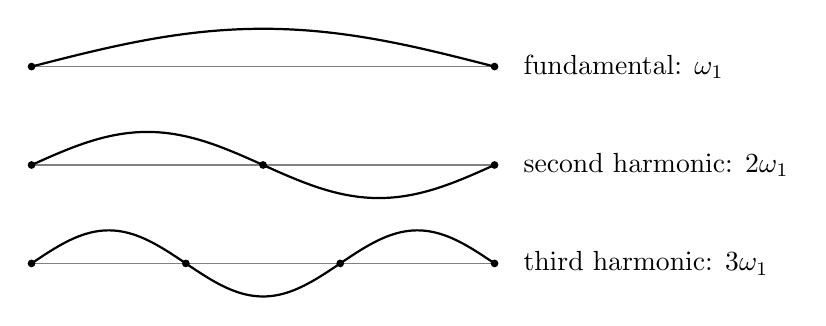
\begin{tikzpicture}[x=0.98cm,y=1cm]
\draw[gray] (0,2.5) -- (6,2.5);
\draw[thick] plot[domain=0:6,samples=120] (\x,{2.5+0.48*sin(30*\x)});
\fill (0,2.5) circle (1.4pt);
\fill (6,2.5) circle (1.4pt);
\node[right] at (6.25,2.5) {fundamental: \(\omega_1\)};

\draw[gray] (0,1.25) -- (6,1.25);
\draw[thick] plot[domain=0:6,samples=120] (\x,{1.25+0.42*sin(60*\x)});
\fill (0,1.25) circle (1.4pt);
\fill (3,1.25) circle (1.4pt);
\fill (6,1.25) circle (1.4pt);
\node[right] at (6.25,1.25) {second harmonic: \(2\omega_1\)};

\draw[gray] (0,0) -- (6,0);
\draw[thick] plot[domain=0:6,samples=120] (\x,{0.42*sin(90*\x)});
\fill (0,0) circle (1.4pt);
\fill (2,0) circle (1.4pt);
\fill (4,0) circle (1.4pt);
\fill (6,0) circle (1.4pt);
\node[right] at (6.25,0) {third harmonic: \(3\omega_1\)};
\end{tikzpicture}%
}
\caption{弦の基本音とその第2倍音および第3倍音。内部節点はそれぞれ0個、1個、2個である。}
\end{figure}

基本音は1つの広いアーチとして動き、内部節点をもたない。それは1つの振動子であり、\(n_1=0,1,2,\ldots\) 個の量子を含みうる。各励起には \(\hbar\omega_1\) のコストがかかる。第2倍音は内部節点を1つもち、振動数は2倍である。基本音が中央ハに聞こえるなら、このモードは1オクターブ高いハに聞こえる。それは独立な占有数 \(n_2\) をもち、その量子の各々には \(\hbar\omega_2=2\hbar\omega_1\) のコストがかかる。第3倍音は内部節点を2つもち、基本振動数の3倍である。それはそれ自身の独立な占有数 \(n_3\) をもち、これもまた任意の非負整数でありうる。

モードごとに、上で用いたエネルギー規約では、エネルギーは占有数に量子エネルギーを掛けたものである。それらの寄与を集めると
\begin{equation}
E=\sum_{N=1}^{\infty} n_N\hbar\omega_N.
\end{equation}
\editorialnote{この表示された和は、01 において別々に述べられたモードエネルギーの代数的な集約である：44：02--01：47：46。}

同じ調和振動子の数学を、すべての場のモードについて繰り返さなければならない。各独立な振動子に対して1つの生成演算子と1つの消滅演算子をもつ。この最初の初等的な描像では、量子場とはその振動子全体の集まりとそれらの生成--消滅代数である。

この言語は粒子散乱に適している。確定したエネルギーと運動量をもつ量子が実験に入り、別のエネルギーと運動量をもつ量子が実験から出ていく。入射粒子は消滅演算子によって取り除かれ、出ていく粒子は対応するモードの生成演算子によって終状態に挿入される。

\begin{classroomqa}
\lecturetimestamp{01:49:38}
\audiencequestion{振動子モードにラベルを付けるのと、その中にある量子の数を数えるのに、同じ整数が使われているのか。}
\lecturerresponse{二つの異なる整数がある。モードラベル\(N\)は空間的パターンを特定する。弦の例では、その節の数が振動数\(\omega_N\)を決める。占有数\(n_N\)は、その振動数をもつ量子がいくつあるかを示す。}
\end{classroomqa}